We show how to program the Vaman FPGA/microcontroller board.  

%ॐ श्री गणेशाय नमः॥
%\\
%\indent जय श्री राम।
%This manual provides a simple introduction to Digital Design.

%\section{Nomenclature}
%\printnomenclature[1.7in]
%%\addcontentsline{toc}{chapter}{Nomenclature}

%\nomenclature{Seven Segment Display}{ सप्तांश प्रदर्शी} 
%\nomenclature{Code}{ गूढ़} 
%\nomenclature{Decoder}{ गूढ़वाचक}
%\nomenclature{Incrementing}{ परवर्ती}
%\nomenclature{Decrementing}{ पूर्ववर्ती}
%\nomenclature{Karnaugh Map}{ कार्नो मानचित्र}
%\nomenclature{Implicant}{ विवक्षक}
%\nomenclature{LED}{ प्रकाश उत्सर्जक यंत्र}
%\nomenclature{Table}{ सारणी}
%\nomenclature{Figure}{ आकृति}
%\nomenclature{Variable}{ चर}
%\nomenclature{Input}{ आगत}
%\nomenclature{Output}{ निर्गत}
%\nomenclature{Boolean Algebra}{ बूलीय बीजगणित}
%\nomenclature{Verify}{ सत्यापित}
%\nomenclature{Combinational Logic}{ संयोजक तर्क}
%\nomenclature{Minimize}{ कनिष्ठीकरण}
\nomenclature{Execute}{ निष्पादित, चालयन}
%\nomenclature{Expression}{ व्यंजक}
%\nomenclature{Equation}{ समीकरण}
%\nomenclature{Axiom}{ अभिगृह}
%\nomenclature{Reduced}{ समानयनिक}
%\nomenclature{C Program}{ C क्रमादेश}
\nomenclature{Programming}{  क्रमादेशन}
%\nomenclature{Frequency}{ आवृत्ति}
\nomenclature{Wordlength }{ मात्राभार}
%\nomenclature{Cable}{ रज्जु}
%\nomenclature{Button}{ गण्ड}
%\nomenclature{Left}{ वाम}
%\nomenclature{Right}{दक्षिण}
%\nomenclature{Blink}{श्मील}
%\nomenclature{IP Address}{अनिकेत}
%\nomenclature{Send}{प्रेषण}
%\nomenclature{File}{सञ्चिका}
%\nomenclature{Setup}{सप्रतिष्ठान}
%\nomenclature{Execute}{चालयन}
%\nomenclature{Interval}{अंतराल}

%\nomenclature{Binary}{ द्विआधारी}
%\nomenclature{Truth Table}{सत्य सारणी}
%\nomenclature{Derive}{व्युत्पन्न }
%\nomenclature{XOR}{अर्ध योग}
%\nomenclature{Complement}{पूरक}
%\nomenclature{Decade Counter}{दशक गणित्र}
%\nomenclature{Digital Logic}{अंकीय तर्क}
%\nomenclature{Function}{फलन}
%\nomenclature{Block Diagram}{खण्डारेख}
%\nomenclature{Circuit}{परिपथ}
%\nomenclature{Simplified Expression}{सरलीकृत व्यंजक}
%\nomenclature{Delay}{अतिकाल}
%\nomenclature{Minute}{निमिश}
%\nomenclature{Synchronous}{तुल्यकालिक}
\nomenclature{Finite State Machine}{परिमित अवस्था यंत्र}
%\nomenclature{State Transition Table}{अवस्थान्तरण सारणी}
%\nomenclature{Flip flop}{द्विविध}
%\nomenclature{Design}{अभिकल्प}
%\nomenclature{Implementation}{कार्यान्वयन}
%\nomenclature{Period}{आवर्त}
\nomenclature{Hardware}{यंत्रान्श}
\nomenclature{Software}{तंंत्रान्श}
\nomenclature{Computer}{संगणक}
%\nomenclature{Board}{परिपथफलक}
%\nomenclature{Port}{पत्तन}
\nomenclature{Now}{इदान}
\nomenclature{Weblink}{जालबन्धन}
\nomenclature{Download}{अवाहरत}
\nomenclature{Resistance}{प्रतिरोध}
\nomenclature{Flash}{प्रस्फुरण}
\nomenclature{Permutation}{क्रमचय}
\nomenclature{Combination}{संचय}
\nomenclature{Sequential Circuit}{अनुक्रमिक परिपथ}







 

%
\begin{enumerate}[label=\arabic*.,ref=\theenumi]
	\item Follow the instructions available in the video at
\begin{lstlisting}
https://github.com/whyakari/TermuxDisableProcces?tab=readme-ov-file
\end{lstlisting}
to ensure that termux is not killed during the following installation process.
\item On termux-debian,
\begin{lstlisting}
wget https://raw.githubusercontent.com/gadepall/fwc-1/main/scripts/setup.sh
bash setup.sh
\end{lstlisting}
%
\item Login to termux-debian on the android device and execute the following commands
\begin{lstlisting}
cd vaman/fpga/setup/codes/blink
source ~/.vamenv/bin/activate
ql_symbiflow -compile -src vaman/fpga/setup/codes/blink -d ql-eos-s3 -P PU64 -v helloworldfpga.v -t helloworldfpga -p pygmy.pcf -dump binary
scp blink/helloworldfpga.bin pi@192.168.0.114:
\end{lstlisting}
Make sure that the appropriate IP address for the raspberry pi is given in the above command.
\item Put the Vaman board in download mode.  For this, you need to first press the button to the right of the usb port and immediately press the button to the left.  The green led should now flash and you can go to the next step.  
\item Now execute the following commands on the raspberry pi.
\begin{lstlisting}
python3 -m venv ~/.vamenv
source ~/.vamenv/bin/activate
git clone --recursive https://github.com/QuickLogic-Corp/TinyFPGA-Programmer-Application.git
pip3 install tinyfpgab
deactivate
sudo reboot
source ~/.vamenv/bin/activate
python3 TinyFPGA-Programmer-Application/tinyfpga-programmer-gui.py --port /dev/ttyACM0 --appfpga /home/pi/helloworldfpga.bin --mode fpga --reset
\end{lstlisting}
\item Make sure that the correct USB port address is given in the above command.    After some time, the LED will start blinking red.
\item Replace  the following line in the code in instruciton  \ref{eq:vaman/fpga/setup/program} 
\begin{lstlisting}
assign redled = led; //If you want to change led colour to red,
\end{lstlisting}
with
\begin{lstlisting}
assign blueled = led; 
\end{lstlisting}
and execute the code.
\item In the following .pcf file,
\begin{lstlisting}
codes/blink/pygmy.pcf
\end{lstlisting}
the pin numbers for the 3 colour-leds are defined.  See 
\autoref{tab:vaman/esp32/setup/onboard}
and
\autoref{fig:vaman/fpga/sevenseg/pins}.  The IO locations in 
		\autoref{fig:vaman/fpga/sevenseg/pins} can be found in pygmy.pcf while the aliases (GPIO) are printed on the board.
\item Now modify the helloworldfpga.v  file to get the green led blinking.
\item In the following verilog program, 
\label{eq:vaman/fpga/setup/program}
\begin{lstlisting}
codes/blink/helloworldfpga.v
\end{lstlisting}
pay attention to the following lines
%%
\begin{lstlisting}
delay = delay+1;                                                                                                   
if(delay > 20000000)
begin
delay=25'b0;
led=!led;
end
\end{lstlisting}
%%
It may be deduced from the above that the blink frequency is 20 MHz.
\item In instruction  \ref{eq:vaman/fpga/setup/program}, replace
\label{eq:vaman/fpga/setup/binary}
\begin{lstlisting}
if(delay > 20000000)
\end{lstlisting}
%
with
\begin{lstlisting}
if(delay==25'b1001100010010110100000000)
\end{lstlisting}
and execute the verilog code.
\item Since the delay is 20 MHz, the blink period is 1 second.  Modify the verilog code
so that the blink period becomes 0.5s.
\item Find the bit length of 20 MHz.
\\
\solution 
\begin{align}
\log_2\brak{20000000} \approx 25
\end{align}
\item Obtain the above answer using a Python code.
\\
\solution Execute the following code and compare with instruction  \ref{eq:vaman/fpga/setup/binary}.
\begin{lstlisting}
codes/blink/freq_count.py
\end{lstlisting}
\item Ensure that the LED stays on in green colour.
	\\
\solution  Execute the following code
\begin{lstlisting}
vaman/setup/codes/blink/onoff.v
\end{lstlisting}
\item Execute the following code and make pin connections as per
\autoref{tab:vaman/fpga/setup/input}.
	Take out the input pin connect to 3.3V. Plug it again.
Do this repeatedly.
\begin{lstlisting}
vaman/setup/codes/input/blink_ip.v
vaman/setup/codes/input/pygmy.pcf
\end{lstlisting}
\begin{table}[]
\centering
\begin{tabular}{|l|l|l|}
\hline
Type & Vaman Pin  &  Connection \\ \hline
Input &  IO\_28 &  3.3V \\ \hline
%Output  & IO\_11  &  LED\\ \hline
\end{tabular}
\caption{Vaman Input/Output.}
\label{tab:vaman/fpga/setup/input}
\end{table}
\item Connect an external LED and repeat.
%
\begin{figure*}[!ht]
\centering
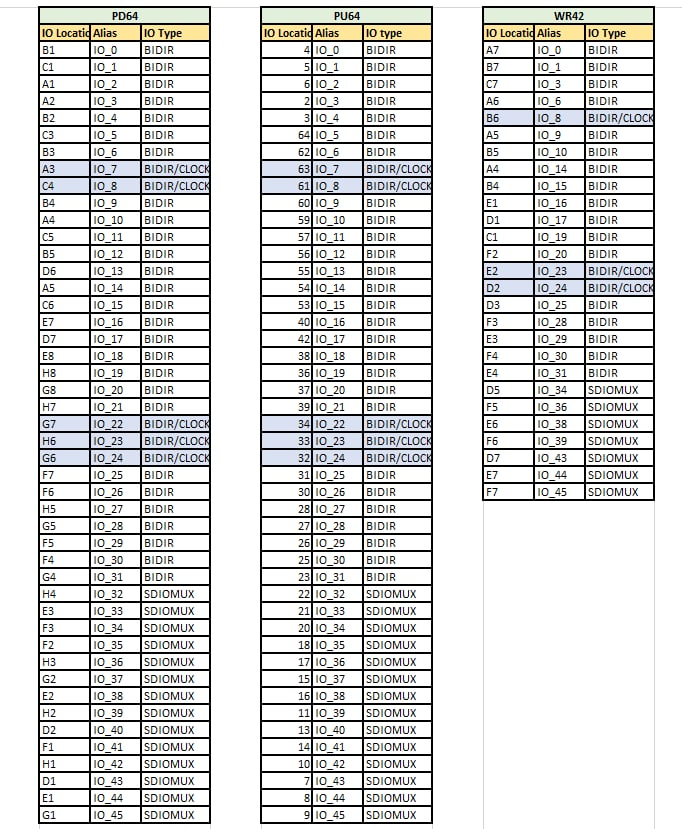
\includegraphics[width = \textwidth]{vaman/fpga/sevenseg/figs/pins.jpg}
\caption{Pin Definitions}
\label{fig:vaman/fpga/sevenseg/pins}
\end{figure*}

\iffalse
\item  Table \ref{table:sevenseg} and
the PU 64 table in Fig. \ref{fig:vaman/fpga/sevenseg/pins}  explain the pin numbering in the following file.
\begin{lstlisting}
codes/static/Vaman.pcf
\end{lstlisting}
\item  Using \autoref{tab:vaman/fpga/setup/input} and
\autoref{fig:vaman/fpga/sevenseg/pins}, control the onboard LED
through an external input. 
\fi



\end{enumerate}

